
% Use the following line  only  if you're still using LaTeX 2.09.
%\documentstyle[icml2014,epsf,natbib]{article}
% If you rely on Latex2e packages, like most moden people use this:
\documentclass{article}

% use Times
\usepackage{times}
% For figures
\usepackage{graphicx} % more modern
%\usepackage{epsfig} % less modern
\usepackage{subfigure} 

% For citations
\usepackage{natbib}
\usepackage{comment}

% For algorithms
\usepackage{algorithm}
\usepackage{algorithmic}

% As of 2011, we use the hyperref package to produce hyperlinks in the
% resulting PDF.  If this breaks your system, please commend out the
% following usepackage line and replace \usepackage{icml2014} with
% \usepackage[nohyperref]{icml2014} above.
\usepackage{hyperref}

% Packages hyperref and algorithmic misbehave sometimes.  We can fix
% this with the following command.
\newcommand{\theHalgorithm}{\arabic{algorithm}}

% Employ the following version of the ``usepackage'' statement for
% submitting the draft version of the paper for review.  This will set
% the note in the first column to ``Under review.  Do not distribute.''
%\usepackage{icml2014} 
% Employ this version of the ``usepackage'' statement after the paper has
% been accepted, when creating the final version.  This will set the
% note in the first column to ``Proceedings of the...''
\usepackage[accepted]{icml2014}



\begin{document} 

\twocolumn[
\icmltitle{Recurrent neural network as a language model - technical report}

\icmlauthor{Wojciech Zaremba}{woj.zaremba@gmail.com}
\icmladdress{New York University}
\icmlauthor{Rob Fergus}{fergus@cs.nyu.edu}
\icmladdress{New York University}
\vskip -0.12in
\icmladdress{Facebook AI Group}

\icmlkeywords{natual language processing, recurrent neural networks, language model}

\vskip 0.3in
]

\begin{abstract} 
  Recurrent neural networks (RNN) offer powerful framework to learn any arbitrary dependency.
  They are expressive as a finite memory Turning machine (e.g. brain). However, their 
  training is difficult, and computationally expensive.


  This work focuses on training RNNs for character level language modelling task. 
  We provide set of pragmatic recommendations about how to train a simple, one layer RNNs 
  for such task.
  Moreover, we support our statements with Theano \cite{bergstra+al:2010-scipy} code which reproduces close to state-of-the-art results
  on Penn Treebank Corpus (code executable both on CPU and GPU). 
\end{abstract} 

\section{Introduction}
Neural networks (NN) are stacked linear transformations alternated with non-linearities. 
Current, state-of-the-art results in many computer vision tasks are achieved with feed-forward neural networks.
In feed-forward networks computation flows in one direction from input layer to output layers.
Recurrent neural networks (RNN) contain connection between instances
of feed forward networks shifted in time. Such connections allow to maintain memory, and perform prediction dependent on
a history. Based on current advances in computer vision thanks to feed-forward networks, we believe
that models heavily utilizing RNNs can bring superior to current state-of-the-art results on NLP tasks.
Moreover, we believe that they might be crucial for further advances in computer vision (attention based models, 
and video prediction). 


Common setting for RNN is a prediction of next element in a sequence. Input is a single element of 
a sequence, and a previous state. 
Consecutive elements of sequence are fetched by RNN. Network attempts at every stage to predict next element of sequence.
We examine such setting on task of language modelling. For purpose of simplicity, we
constrain ourselves to character level language modelling.



Typical training procedure for RNNs is stochastic gradient descent (SGD). However, it is difficult to obtain
a valuable models of RNNs by applying unconstrained SGD.
Recurrency brings much higher expressive power in compare feed-forward networks, and in the same time it makes them more difficult to train. There
are several common issues (1) vanishing gradient, (2) exploding gradient, (3) short memory. We address
exploding gradient issue by clipping gradients, and we don't tackle remaining problems.


We proceed by presenting related work (Section \ref{sec:related work}). Next, we describe our framework (Section
\ref{sec:framework}), and finally we present experimental results (Section \ref{sec:experiments}). 
Code allowing to reproduce experiments (and train any arbitrary RNN on CPU or GPU) is available online\footnote{\url{https://github.com/wojzaremba/rnn}}.

\section{Related work}\label{sec:related work}
There have been expensive interest in different flavours of neural networks 
with recurrent connections \cite{hopfield1982neural, hinton2006fast}. This
approaches consider recurrency not to account for time dependency, but
for internal data dependency (e.g. correlation between pixel values). 


We are mainly interest in RNNs, which aim to predict 
time-dependent sequence. \cite{mikolov2012statistical} 
\cite{sutskever2013training} consider extensively 
training of such networks for characters, and words. Moreover,
they analyze how best optimize such models (e.g. with Hessian-free method, or 
by clipping gradients).


\cite{graves2013generating} focuses on how to extend memory of model. 
He addresses it by using Long-Short-Term-Memory units (LSTSs).
There are weak evidences that LSTMs prevent gradient from vanishing.

\section{Framework}\label{sec:framework}
Our code is build in Theano. This python framework allows to define python symbolic expressions, and 
differentiate with respect to them. Moreover, it compiles code to fast CPU or GPU executable versions.
We present here setup for our best model.


We have trained a simple RNN as depicted on the Figure \ref{fig:schema}. Our best model has 600 hidden units.
We initialized all weights with Gausssian having $0.001$ variance, and all biases with $0$. 
It is good to reset hidden values between different instances of text. It's better to set it to all ones, rather
than to all zeros.
We train model with
SGD on minibatches of size 10, and we unroll RNN for 10 steps. We don't use any momentum (for such small models 
it doesn't make a big difference). We clip gradients above norm $15$ (if norm of a gradient is higher than $15$ then
we project it down).
Our initial learning rate is $0.1$. We decrease it by factor of $2$ every time
when perplexity on a validation set increases (we measure perplexity in every epoch). It takes around $5-8$ epochs
to decrease learning rate. Single epoch computes for $20$ minutes.
If perplexity increased 
for 2 epochs then we finish training (early stopping criteria).



\begin{figure}
  \subfigure[Figure presents information flow in recurrent network based on the simplest possible neural network. 
  Experiments in this paper have been perfomed on such networks, where non-linearity is a sigmoid, and classifier is 
a softmax. We consider models with hidden layers of the size $200, 600, 1000$, and input is always a ASCII character.
Input can be represented as an indicator vector having 256 dimensions, however in practise is better to story it as int8.]{
    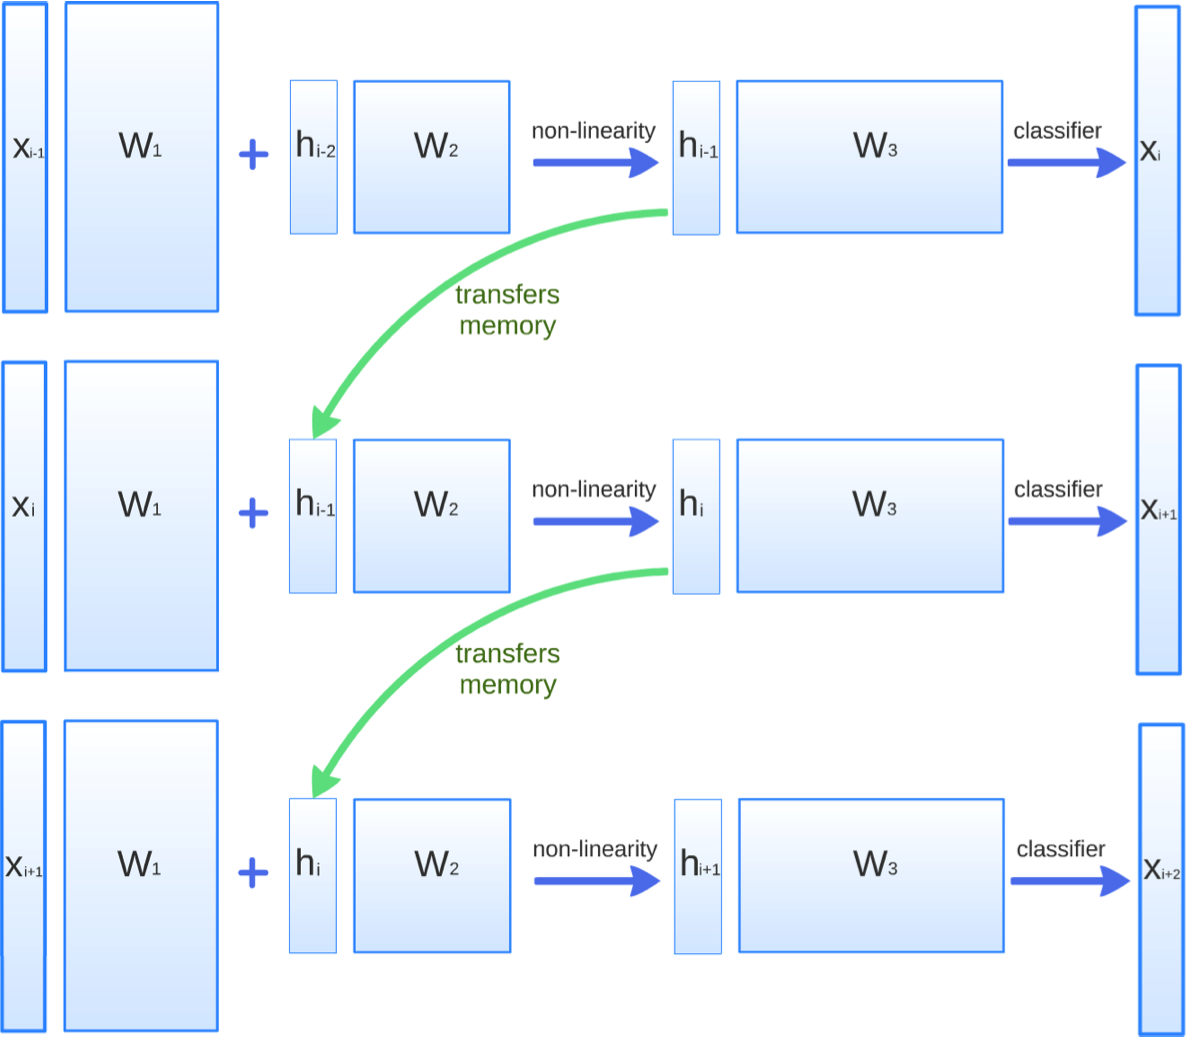
\includegraphics[width=\linewidth]{img/schema.png}
  }\label{fig:schema}
\end{figure}

Final layer is a softmax. This classifier gives probabilities of ocurrence for next character. During sequence generation
, we sample from this probability. 


\section{Experiments}\label{sec:experiments}
First, we designed experiments to verify that our model has any memory. 
Next we trained it Penn Treebank Corpus\footnote{\url{http://www.fit.vutbr.cz/~imikolov/rnnlm/simple-examples.tgz}}.  


\subsection{Synthetic data}
Our first experiment verifies that our model has any memory. I have trained network on sequences ''aabbccddaabbccdd$\dots$`` starting
from any arbitrary random position. In order to give a proper prediction of next character network has to remember what
is the current position. If it is a first ''a``, or a second ''a``. Starting from any random position (with clean hidden state), for first two predictions
network is uncertain about next character. However, after two predictions, all next predictions are deterministic. Network
learns to predict them correctly. Very shortly networks gets perplexity close to one on this task. Moreover, we can condition
on initial part of sentence, and generate rest of it. Tables \ref{tab:a}, \ref{tab:aabb} shows exemplary generated sequences.


\begin{table}[t]
\tiny
\centering
\begin{tabular}{l}
\hline
Generated sequence from input sequence ``a'' \\
\hline
 abbccddaabbccddaabbccddaabbccddaabbccddaabbccddaabbccddaabbccdd\\
 aabbccddaabbccddaabbccddaabbccddaabbccddaabbccddaabbccddaabbccd\\
 aabbccddaabbccddaabbccddaabbccddaabbccddaabbccddaabbccddaabbccd\\
 abbccddaabbccddaabbccddaabbccddaabbccddaabbccddaabbccddaabbccdd\\
 adaabbccddaabbccddaabbccddaabbccddaabbccddaabbccddaabbccddaabbc\\
\hline
\end{tabular}
\caption{Toy example showing that network has memory. As it generates sequences starting from ``a'' there is 
        ambiguity.}
        \label{tab:a}
\end{table}



\begin{table}[t]
\tiny
\centering
\begin{tabular}{l}
\hline
Generated sequence from input sequence ``aabb'' \\
\hline
 aabbccddaabbccddaabbccddaabbccddaabbccddaabbccddaabbccddaabbccd\\
 aabbccddaabbccddaabbccddaabbccddaabbccddaabbccddaabbccddaabbccd\\
 aabbccddaabbccddaabbccddaabbccddaabbccddaabbccddaabbccddaabbccd\\
 aabbccddaabbccddaabbccddaabbccddaabbccddaabbccddaabbccddaabbccd\\
 aabbccddaabbccddaabbccddaabbccddaabbccddaabbccddaabbccddaabbccd\\
\hline
\end{tabular}
\caption{Initial sequence ``aabb'' determines further sequence unambiguously.}
        \label{tab:aabb}
\end{table}



\subsection{Penn Treebank Corpus}
After 24 epochs of training (8h) we have achieved perplexity on the test data 2.94. 
Tomas Mikolov reports perplexity 2.6 on his best model.
Table \ref{tab:penn} presents generated sentences for our model.


\begin{table}[t]
\tiny
\centering
\begin{tabular}{l}
\hline
Generated sequence from input sequence ``My name is'' \\
\hline
 My name is profitable mr. $<$unk$>$ northern new protecting earnings\\ 
 My name is pg according to a roller-based in the world the $<$unk$>$\\
 My name is $<$unk$>$ of primary sales bridge brokers rose N N to N a\\
 My name is playing improve new shareholders fell N N in october \\
 My name issues cud holds of $<$unk$>$ abortion agreement bill one of\\

My name is relatively ms. <unk> hill which i limit it social it can encourage three quake
My name is r. <unk> eurocom <unk> to <unk> more <unk> <unk> 's claims and <unk> that creditors who often appar
My name is <unk> on smaller sales are clearance by long-term alternatives
My name is reinvestment on senate is a voting oil co. his claim of soon by halt to high according to its steel
My name issues culming was having a market acknowledged that it is in the treasury kennedy

\hline
\end{tabular}
\caption{Most of generated words are correct English words. Moreover, they
are combined in close to a grammatical way.}
        \label{tab:penn}
\end{table}


\section{Discussion}
Although language model generated by RNNs is impressive, still it is far from
human generated text. It is crucial to understand what are the missing components
to achieve closer to human performance. It might be optimization problem, or
maybe missing computational unit problem. We would like to understand this challenges
on the large scale dataset both in the context of NLP, as well as computer vision tasks.


\section{Acknowledgment}
Thank you to Ilya Sutskever, Tomas Mikolov, Caglar Gulcehre for insightful discussions on how to train RNNs.

\bibliography{bibliography}
\bibliographystyle{icml2014}

\end{document} 

